  \section{Monitoring}
    \subsection{Qu'est-ce que c'est ?}
      \bframe
        \begin{itemize}
          \item étude bas niveau du comportement matériel et système
          \item très utile pour le débugage ou l'optimisation poussée
          \item différentes solutions de monitoring existent
        \end{itemize}
      \end{frame}

    \subsection{Instruction Based Sampling - Présentation}
      \bframe
        \begin{itemize}
          \item technologie AMD
          \item informations plus précises car spécifique à une famille de
            processeur
          \item problème:
            \begin{itemize}
              \item plus difficile à mettre en place
            \end{itemize} 
        \end{itemize}
      \end{frame}

    \subsection{Instruction Based Sampling - Fonctionnement}
      \bframe
        \begin{itemize}
          \item tag aléatoirement une instruction
          \item suivi de l'exécution
          \item deux types de mesures: fetch/execution sampling
        \end{itemize}
      \end{frame}

    \subsection{Instruction Based Sampling - Utilisation}
      \bframe
        \begin{itemize}
          \item<1-2> beaucoup d'informations remontées par IBS
          \item<1-2> sélection des plus utiles: cache hit/miss
        \end{itemize}

        \visible<2->{
          \begin{figure}[h]
            \centering
            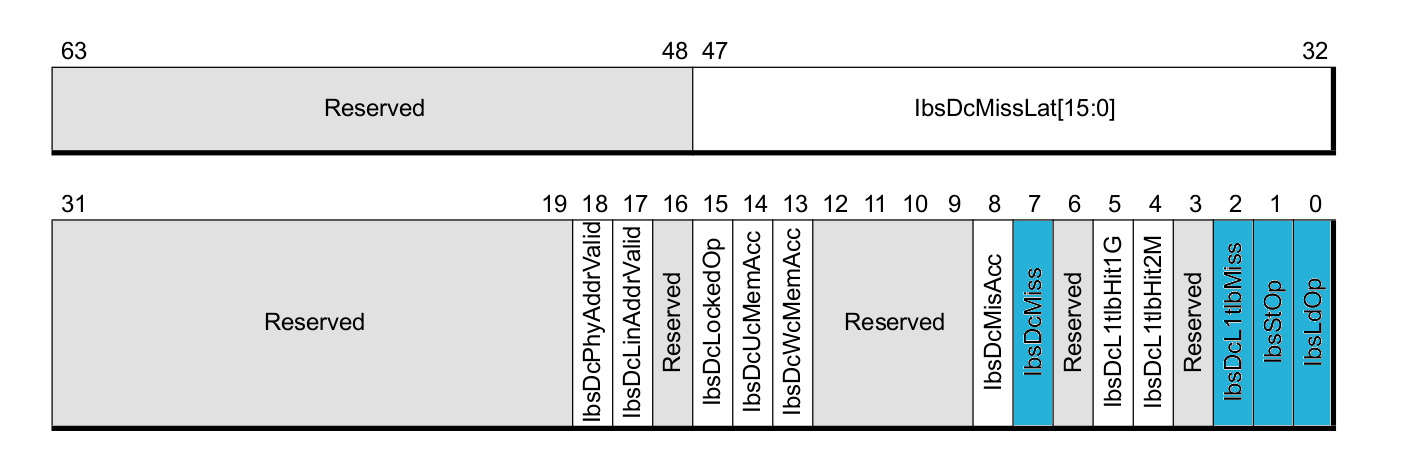
\includegraphics[scale=0.22]{img/data3_color.png}
            \caption{Schéma du registre MSR IbsOpData3}
          \end{figure}
        }
      \end{frame}

    \subsection{Instruction Based Sampling - Défauts}
     \bframe
       \begin{itemize}
         \item overhead: traitement coûteux des mesures
         \item pas de vision d'ensemble
       \end{itemize}
     \end{frame}

    \subsection{Mise en place}
      \bframe
        \begin{itemize}
          \item configuration de l'APIC
          \begin{itemize}
            \item informer l'APIC de la présence d'interruptions IBS
            \item à faire pour chaque coeur
          \end{itemize}
          \item enregistrement d'un handler NMI
          \begin{itemize}
            \item appelé à chaque interruption IBS
            \item récolte les informations dans les registres MSR
          \end{itemize}
        \end{itemize}
        \visible<2->{
          \begin{alertblock}{Attention}
            le handler doit être enregistré une et une seule fois au niveau du système
          \end{alertblock}
        }
      \end{frame}


